Este capítulo descreve a metodologia adotada para investigar a formação e impacto de câmaras de eco na rede de usuários da aplicação Colab. A pesquisa é estruturada de forma iterativa e incremental, permitindo que cada etapa informe e refine as subsequentes.

\section{Natureza da Pesquisa}

A pesquisa adota uma abordagem tanto descritiva quanto exploratória, conforme delineado por \cite{2008_Yin_BOOK} e \cite{2007_Babbie_BOOK}.

A pesquisa descritiva, como sugerido por \cite{2007_Babbie_BOOK}, é empregada quando o objetivo é descrever características de um fenômeno ou a relação entre variáveis. No contexto deste estudo, a abordagem descritiva é utilizada para categorizar e detalhar os usuários do Colab, fornecendo uma representação clara e sistemática dos mesmos. Esta metodologia é particularmente útil para estabelecer um panorama claro do comportamento dos usuários, suas interações e padrões de linguagem, formando assim a base para análises subsequentes.

Por outro lado, a pesquisa exploratória, conforme descrito por \cite{2008_Yin_BOOK}, é frequentemente empregada quando o pesquisador tem pouco ou nenhum conhecimento prévio sobre o fenômeno em estudo. Ela busca descobrir padrões, ideias ou hipóteses, em vez de testar uma hipótese predefinida. No caso desta pesquisa, a abordagem exploratória é crucial para identificar e compreender as câmaras de eco dentro da rede do Colab, um fenômeno ainda pouco explorado na literatura. Esta abordagem permite uma investigação flexível, adaptando-se à medida que novas descobertas emergem.

A combinação dessas duas abordagens é estratégica. Enquanto a pesquisa descritiva fornece uma base sólida e detalhada sobre os usuários e suas interações, a pesquisa exploratória permite a descoberta de novos insights e compreensões sobre as câmaras de eco. Esta combinação maximiza a profundidade e amplitude da análise, garantindo que tanto os aspectos bem definidos quanto os emergentes do fenômeno sejam adequadamente abordados.

A metodologia deste estudo segue uma abordagem sequencial e iterativa, dividida em distintas fases interligadas. Cada fase é projetada para conduzir experimentos específicos que contribuem para uma compreensão mais profunda e abrangente das dinâmicas presentes na rede Colab.

Em cada fase, são definidos objetivos claros e hipóteses a serem testadas. A fase inicial se concentra na coleta e análise descritiva de dados do Colab, visando caracterizar os usuários, eventos e interações. Os resultados dessa fase são fundamentais para estabelecer uma base sólida e compreensível sobre o comportamento dos usuários.

À medida que avançamos para as fases subsequentes, os resultados dos experimentos anteriores são utilizados como insumos essenciais. Por exemplo, os dados coletados na primeira fase, que detalham as interações dos usuários, servem como base para a identificação das comunidades da rede na segunda fase. Os insights obtidos na segunda fase, por sua vez, orientam a seleção de tipos de eventos específicos a serem analisados na terceira fase.

Essa abordagem sequencial e iterativa permite que cada fase da pesquisa se beneficie das descobertas e conclusões anteriores, enriquecendo a análise e possibilitando insights mais profundos. Além disso, essa estratégia promove a construção gradual de conhecimento, à medida que cada experimento agrega informações e levanta novas questões a serem exploradas.

Em resumo, a pesquisa adota uma estratégia de fases interdependentes, em que os resultados de cada experimento alimentam o próximo, ampliando nosso entendimento das dinâmicas da rede Colab e das câmaras de eco presentes nesse ambiente

\section{Universo e Amostra}
Os dados utilizados são oriundos do aplicativo Colab, representando um universo de [X usuários] no período de [data de início] a [data de fim] cobrindo as cidades de Caruaru, Rio de Janeiro, Recife, Niterói, Mesquita e Santo André. Nessa amostragem os usuários realizaram [X postagens] e [X comentários] num total de [X interações] analisadas.

\section{Coleta de Dados}
Os dados foram fornecidos pelo aplicativo Colab em formato CSV. Estes incluem listas de arestas, que representam as conexões entre os usuários, informações sobre o comportamento dos usuários, suas interações e postagens, além de dados demográficos e geográficos. Os dados foram anonimizados e não contêm informações pessoais dos usuários. O modelo dos dados e os preprocessamentos realizados são detalhados no \autoref{sec:modelo_de_dados}.

\section{Procedimentos de Análise}
\begin{itemize}
	\item \textbf{Análise de Redes Sociais:} Utilizando técnicas de ciência de dados e análise de grafos para identificar estruturas e características da rede Colab.
	\item \textbf{Classificação de Usuários:} Serão empregadas técnicas de processamento de linguagem natural e aprendizado de máquina supervisionado para classificar postagens e comportamentos dos usuários.
	\item \textbf{Detecção de Câmaras de Eco:} Adaptação das heurísticas propostas por \cite{2023_Atiqi_BOOK} ao contexto do Colab, combinadas com técnicas de análise de redes e teoria dos grafos.
	\item \textbf{Simulações:} A Modelagem Baseada em Agentes (ABM) e simulações de Monte Carlo serão usadas para avaliar o impacto de diferentes cenários e intervenções na formação de câmaras de eco.
\end{itemize}

\begin{figure}
	\centering
	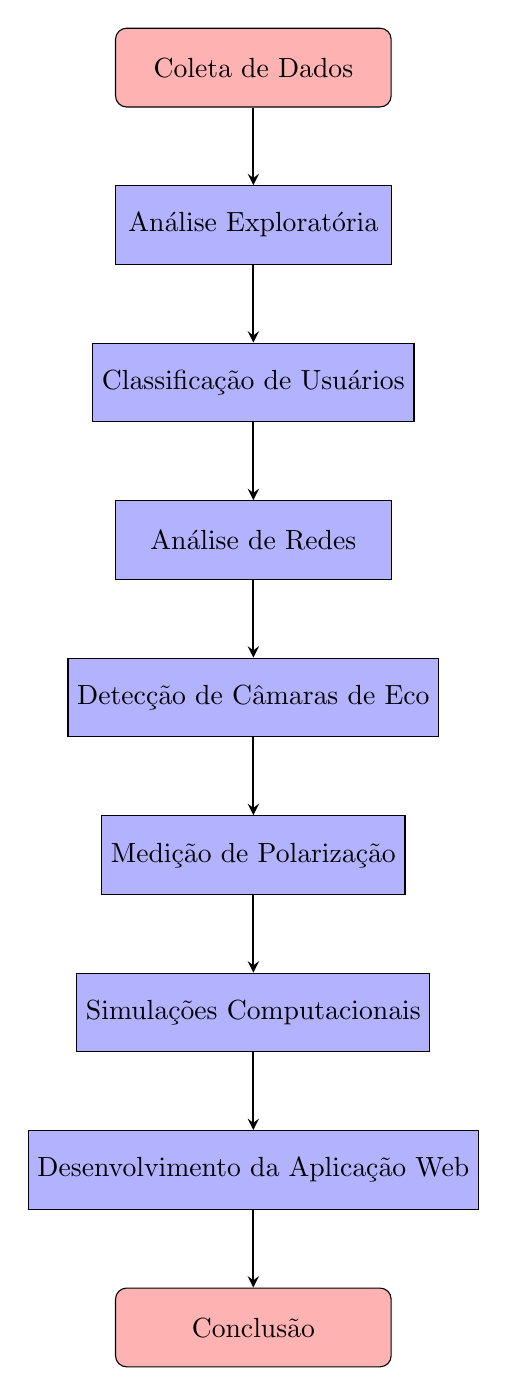
\begin{tikzpicture}[node distance=2cm]
		% Estilos para os nós
		\tikzstyle{startstop} = [rectangle, rounded corners, minimum width=3.5cm, minimum height=1cm, text centered, draw=black, fill=red!30]
		\tikzstyle{process} = [rectangle, minimum width=3.5cm, minimum height=1cm, text centered, draw=black, fill=blue!30]
		\tikzstyle{arrow} = [thick,->,>=stealth]
		% Nós
		\node (start) [startstop] {Coleta de Dados};
		\node (proc1) [process, below of=start] {Análise Exploratória};
		\node (proc2) [process, below of=proc1] {Classificação de Usuários};
		\node (proc3) [process, below of=proc2] {Análise de Redes};
		\node (proc4) [process, below of=proc3] {Detecção de Câmaras de Eco};
		\node (proc5) [process, below of=proc4] {Medição de Polarização};
		\node (proc6) [process, below of=proc5] {Simulações Computacionais};
		\node (proc7) [process, below of=proc6] {Desenvolvimento da Aplicação Web};
		\node (stop) [startstop, below of=proc7] {Conclusão};
		% Setas
		\draw [arrow] (start) -- (proc1);
		\draw [arrow] (proc1) -- (proc2);
		\draw [arrow] (proc2) -- (proc3);
		\draw [arrow] (proc3) -- (proc4);
		\draw [arrow] (proc4) -- (proc5);
		\draw [arrow] (proc5) -- (proc6);
		\draw [arrow] (proc6) -- (proc7);
		\draw [arrow] (proc7) -- (stop);
	\end{tikzpicture}
	\caption{Diagrama ilustrando os passos da metodologia.}
\end{figure}

\section{Ferramentas e Softwares}

Análise Exploratória de Redes com Gephi: Inicialmente, será conduzida uma análise exploratória de redes usando o software Gephi. Esta fase permitirá visualizar a estrutura da rede, identificar clusters e comunidades e também entender os padrões de interação entre os usuários.

Análise de Redes com Python e NetworkX: Para um exame mais detalhado e uma análise quantitativa da rede, utilizaremos Python, especificamente a biblioteca NetworkX. Com isso, esperamos identificar métricas-chave da rede, como centralidade, densidade e modularidade. Esse estudo nos ajudará a identificar as câmaras de eco e seus nós principais.

Modelagem Baseada em Agentes: A modelagem baseada em agentes será empregada para simular o comportamento dos usuários e a propagação de informações. Isso nos permitirá prever a propagação de informações dentro e entre câmaras de eco e tentar entender as dinâmicas que levam à formação de tais câmaras.

Ambiente de Desenvolvimento Google Colaboratory: Todas as análises computacionais e o desenvolvimento de algoritmos serão realizados no ambiente Google Colaboratory, que oferece um ambiente de codificação interativo e colaborativo baseado na nuvem. Isso facilitará a reproducibilidade da pesquisa e também a colaboração com outros pesquisadores.

\section{Aspectos Éticos}
A pesquisa garante a anonimidade das informações pessoais dos usuários. Todos os dados sensíveis serão tratados com precaução, assegurando a integridade e privacidade dos participantes.

\section{Limitações}
Os resultados e conclusões desta pesquisa são específicos do universo do Colab, o que pode limitar sua generalização para outras plataformas ou contextos.